\section{Motivation for Demand Management}
\label{strategies}

In this section, we motivate the need for demand management and make the case for a tighter integration and communication between ESPs and SCs. We also define \emph{strategies, programs, and methods}, which are techniques for demand management. 

Figure \ref{fig:seq} depicts data collected at three-minute intervals over three days from the Sequoia supercomputer, which is the world's third fastest supercomputer. Sequoia is a 16.3 petaflops that is hosted at LLNL. The y-axis is the power consumed, and the x-axis represents the time samples. As can be noted from this figure, fluctuations of a few megawatts are fairly common. Some of these fluctuations may be related to maintenance cycles and could be scheduled. However, there are other times where the fluctuations are not scheduled in advance and may occur as a result of the workload that is executing on the supercomputer. This data clearly indicates that the SCs should forecast and communicate with their ESPs more often to discuss and address such power swings. \\

\begin{figure}
\begin{center}
\frame{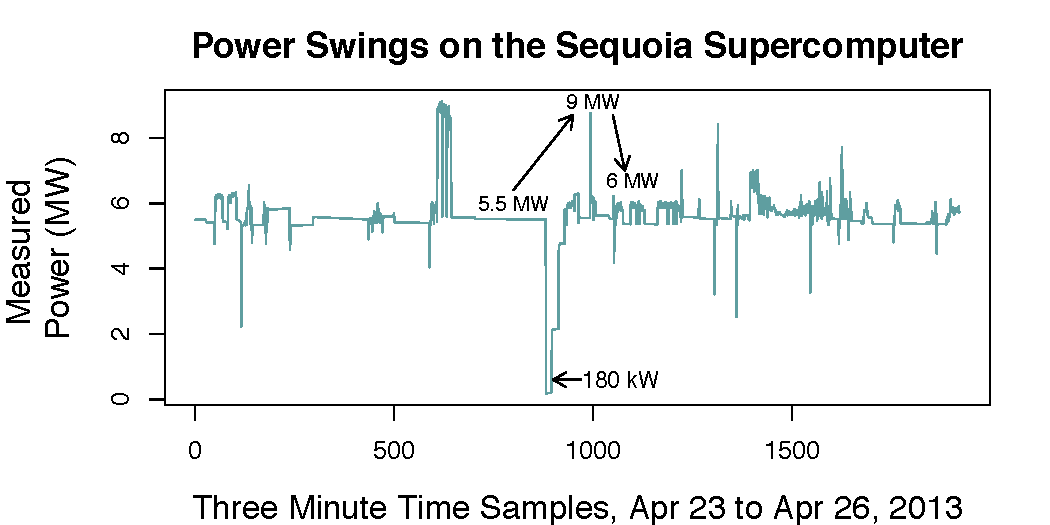
\includegraphics[scale=0.6]{figs/seq.pdf}}
\caption{Sequoia Supercomputer Power Swings}
\label{fig:seq}
\end{center}
\end{figure}

We observe similar trends with data from Titan, which is a supercomputer hosted at ORNL. TODO graph + analysis. \\


We now explain the techniques used in demand management. We define \emph{strategies} as power management techniques used by SCs to manage power. Strategies may or may not improve energy efficiency. For example, \emph{Load Migration} is a strategy that SCs may use in response to an ESP's request, and while it helps manage power effectively, it does not impact the energy efficiency of the site. On the other hand, fine-grained power management techniques, such as using node-level power capping, or better job scheduling algorithms are likely to improve energy efficiency but may not be as useful in response to an ESP request. Almost all sites employ some power management strategies, especially the ones involving lighting, temperature, cooling, fine-grain power management and job scheduling. There is moderate interest in grid integration strategies in the United States, and low interest in the same in Europe. From the point of view of SCs, strategies such as cutting jobs or load migration have little interest. \\

\emph{Programs} are incentives offered by ESPs to their customers and to SCs in order to motivate them to help balance the electrical grid. Common examples include peak shedding, peak shifting and dynamic pricing. From our questionnaire, we concluded that neither European nor the United States sites are engaged with peak shedding, peak shifting or dynamic pricing programs at present. More sites in the United States have communicated with their ESPs regarding these programs. While both European and United States SCs are interested in dynamic pricing, there is mixed interest in peak shedding and peak shifting. The European sites are more interested in peak shedding than peak shifting, but the United States sites are more interested in peak shifting. \\

\emph{Methods} are used by the ESPs to balance the electrical grid in the transmission and distribution phases. Examples of methods include regulation, frequency response, grid scale storage and use of renewable sources of energy. Both European and US sites are interested in discussing renewables with their ESPs, but there is little interest in communicating with regards to the other possible methods. \\

We also asked our European respondents to indicate what might motivate them to communicate with their ESPs. The results are shown in Table \ref{fig:table2}. As can be noted from this figure, the main motivators are the financial incentives and the desire to be ``good citizens.''

\begin{table}[h]
\begin{center}
\begin{tabular}{|l|c|c|c|c|}
\hline
\multicolumn{5}{|p{.72\textwidth}|}{\emph{Ques:} Please evaluate as high, medium or low the following motivations for your site's interest in pursuing a stronger relationship with your electricity service provider}\\
\hline
& Low & Medium & High & Rating Count \\
\hline
Economically justified & 14.3\% (1) & 28.6\% (2) & 57.1\% (4) & 7 \\
\hline
Good citizen & 14.3\% (1) & 71.4\% (5) & 14.3\% (1) & 7 \\
\hline
Adverse consequences & 66.7\% (4) & 16.7\% (1) & 16.7\% (1) & 6 \\
\hline
Government regulation & 71.4\% (5) & 28.6\% (2) & 0.0\% (0) & 7 \\
\hline
\end{tabular}
\end{center}
\caption{Motivation for communicating with ESP (European Respondents)}
\label{fig:table2}
\end{table}
%\begin{figure}
%\begin{center}
%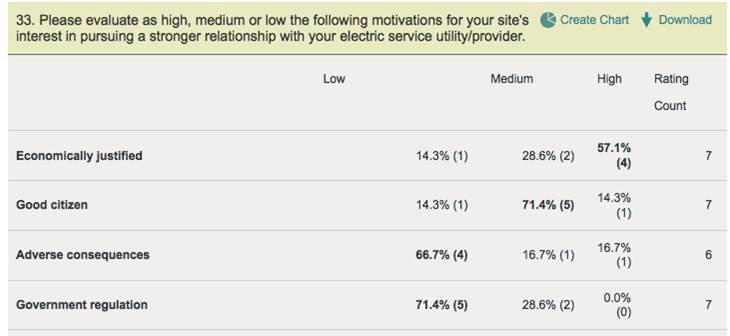
\includegraphics[scale=0.5]{figs/Table2.jpg}
%\caption{Motivation}
%\label{fig:table2}
%\end{center}
%\end{figure}
%
